\documentclass[10pt,letterpaper,xcolor=dvipsnames,handout]{beamer}

%\usepackage[colorlinks=true,linkcolor=blue]{hyperref}
\usepackage{amssymb,mathabx}
\usepackage{linguex}
\usepackage{verbatim,enumerate,multirow}
\usepackage{xcolor}
%\usepackage{floatflt}

\usepackage{pgfpages} % to put several slides on one page
\pgfpagesuselayout{4 on 1}[letterpaper, landscape, border shrink=5mm]

\mode<article>{}

%Template themes
\usetheme{boxes}
%\useoutertheme{miniframes}
\useoutertheme{shadow}

%Templates
\setbeamertemplate{blocks}[rounded][shadow=true]
\setbeamertemplate{navigation symbols}[vertical]
\setbeamertemplate{section in head/foot shaded}[default][20]
\setbeamertemplate{title}

\setbeamertemplate{headline}
{
	\begin{beamercolorbox}[ht=3ex,dp=1ex]{erikcolor1}
		\insertshorttitle
		%\insertsectionnavigationhorizontal{\textwidth}{}{}
		\usebeamerfont{title in head/foot}
	\end{beamercolorbox}
	\begin{beamercolorbox}[ht=3ex,dp=2ex]{erikcolor2}
	  \insertsectionnavigationhorizontal{\textwidth}{}{}
		%\insertsubsectionnavigationhorizontal{\textwidth}{}{}
		%\insertsubsection
	\end{beamercolorbox}
}
\setbeamertemplate{footline}
{
	\begin{beamercolorbox}[ht=3ex,dp=1ex]{erikcolor1}
		\insertshortinstitute[width=.33\textwidth,center] %$\triangleright$
		\insertshortsubtitle[width=.33\textwidth,center] %$\triangleright$
		\insertshortdate[width=.20\textwidth,center] %$\triangleright$
		\hfill\insertframenumber\,/\,\inserttotalframenumber\;\;\;
	\end{beamercolorbox}
}

%Font themes
\usefonttheme{structuresmallcapsserif}
%\usefonttheme[onlysmall]{structurebold}
\usefonttheme{serif}

%Color themes
%\usecolortheme{beetle}
%\usecolortheme{rose}

%Head and foot lines colors
\setbeamercolor{erikcolor1}{fg=white,bg=blue!70!green}
\setbeamercolor{erikcolor2}{fg=white,bg=blue!60!green!10!white}

%Titles color
\setbeamercolor{frametitle}{fg=black,bg=green!30!blue!30!white}
\setbeamercolor{title}{fg=black,bg=green!30!blue!30!white}

%Block color
\setbeamercolor{block title}{fg=white,bg=blue!70!green}
\setbeamercolor{block body}{fg=black,bg=green!30!blue!30!white}

%Background color
\setbeamercolor{background canvas}{bg=}

%Covered items color
\setbeamercovered{transparent}

\AtBeginSection[]
{
   \begin{frame}<beamer>
       \frametitle{Lecture plan}
       \tableofcontents[currentsection,currentsubsection]
   \end{frame}
}



\title{Informal fallacies}
\subtitle{Presumption, ambiguity, transference}
\author[Hoversten]{Erik Hoversten}
\institute[lrp-f14]{Logic, reason, and persuasion: fall 2014 \\ Rutgers University}
\date[09/25/2014]{September 25, 2014}

\begin{document}

\begin{frame}
\titlepage
\end{frame}

\section{Weak induction (cont.)}

\begin{frame}
  \frametitle{Weak analogy}
  
  \begin{block}{False similarity}
    \begin{itemize}
      \item If there is something about which a person is unfamiliar, a good way to describe it to them is by comparing it to something with which they are familiar.
      \item But things can be similar in one way without thereby being similar in other ways.
      \item So, analogies must show a variety of representative similiarities in order to be considered strong.
      \item Compare to hasty generalization
    \end{itemize}
  \end{block}
  
    \begin{center}
    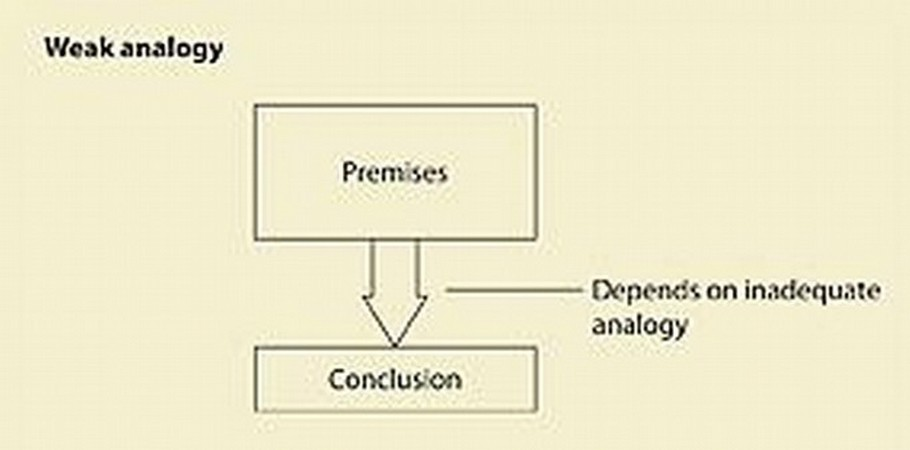
\includegraphics[width=.5\textwidth]{weak-analogy.jpg}
  \end{center}
  
\end{frame}

\begin{frame}
  \frametitle{Weak analogy}
  \framesubtitle{Examples}
  
  \begin{block}{Not much similarity}
    ``Bertha loves living in Brooklyn.  Jim and Bertha are both into food blogs, so I bet Jim would love living in Brooklyn, too.''
  \end{block}
  
  \begin{block}<2->{Non-diverse similarity}
    ``Fred and Gabe are both over six feet, lift weights, and played sports in high school, and Fred got an A in physics.  My money is on Gabe to be pretty good at physics.''
  \end{block}
  
\end{frame}

\section{Fallacies of presumption}

\begin{frame}
\frametitle{Fallacies of presumption}

When one commits a fallacy of this type, they rely on (presume) a piece of information (a proposition) that is either left implicit or unsupported.  Generally, the arguer uses language as a means of hiding the presumed proposition.

We can often reveal the fallacy by making the implicit proposition an explicit premise in our reconstruction of the argument.

\begin{block}{Types}
  \begin{itemize}
    \item Begging the question
    \item Complex question
    \item False dichotomy
  \end{itemize}
\end{block}

\end{frame}

\begin{frame}
  \frametitle{Begging the question}
  \small
  
  \begin{block}{Circular reasoning}
    \begin{itemize}
      \item The purpose of the premises in an argument is to provide the \textit{support} for the conclusion.
      \item But the support they provide must be \textbf{independent} of the conclusion.
      \item When an arguer begs the question, they presume the truth of the conclusion within the premises of their argument.
      \item The result is that the conclusion is used to support itself, but that amounts to nothing more than just stating that the conclusion is true.
    \end{itemize}
  \end{block}
  
  
  \begin{center}
    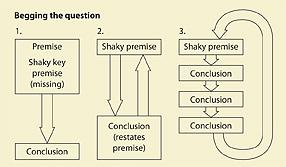
\includegraphics[width=.5\textwidth]{begging.jpg}
  \end{center}
  
\end{frame}

\begin{frame}
  \frametitle{Begging the question}
  \framesubtitle{Examples}
  
  \begin{block}{Restatement of conclusion}
    ``No philosopher would lie in a published work for the simple reason that that would make the philosopher a liar.''
  \end{block}
  
  \begin{block}<2->{Extended circle}
    ``Picasso is the greatest artist of the twentieth century.  We know this because art critics have described him in these terms. We can trust the art critics because they have a more keenly developed sense of taste than most people. This is clear, because it takes a morekeenly developed sense of taste to recognize that Picasso is the greatest artist of the twentieth century.''
  \end{block}
  
\end{frame}

\begin{frame}
  \frametitle{Complex question}
  
  \begin{block}{Damned if you do, damned if you don't}
    \begin{itemize}
      \item The arguer makes as if they are asking a simple question.
      \item But their question presumes the truth of a different question that is controversial.
      \item If you respond to the question, you seem to accept the presumption, and thus come across as guilty either way.
    \end{itemize}
  \end{block}
  
  
  \begin{center}
    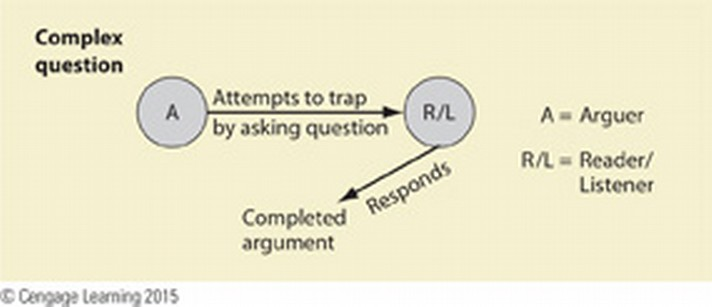
\includegraphics[width=.5\textwidth]{complex.jpg}
  \end{center}
  
\end{frame}

\begin{frame}
  \frametitle{Complex question}
  \framesubtitle{Examples}
  
  \begin{block}{Suscpicious parent to child}
    ``So, who did you get to help you clean up after the party you weren't supposed to have?''
  \end{block}
  
  \begin{block}<2->{Accusatory gossiper}
    ``Isn't that the guy who left his kid to fend for himself in a park all afternoon?''
  \end{block}
  
\end{frame}

\begin{frame}
  \frametitle{False dichotomy}
  
  \begin{block}{Excluded third option}
    \begin{itemize}
      \item We've already introduced the notion of the disjunctive syllogism, which is a valid form of deductive argument.
      \item But the disjunction involved in the argument presumes that the two options it presents are \textbf{exhaustive}.
      \item If there is actually a third option available, then the argument is fallacious.
    \end{itemize}
  \end{block}
  
  \begin{block}<2->{Disjunctive syllogism}
    \begin{enumerate}
      \item $A$ or $B$ (presumption: ``no $C$ option'')
      \item not-$A$
      \item $\therefore$, $B$
    \end{enumerate}
  \end{block}
  
\end{frame}

\begin{frame}
  \frametitle{False dichotomy}
  \framesubtitle{Examples}
  
  \begin{block}{Choice of abstaining}
    ``You're either with us, or you're against us. The senator is clearly not with us.  So he is out to destroy us.  We must fight back!''
  \end{block}
  
  \begin{block}<2->{Non-fallacious disjunctive syllogism}
    \begin{itemize}
      \item A: ``I remember that Kierkegaard either wrote \textit{Fear and Trembling} or \textit{Fear and Loathing}.''
      \item B: ``\textit{Fear and Loathing in Las Vegas} was Hunter S. Thompson's crazy drug trip story.''
      \item A: ``Ok, then Kierkegaard's book was \textit{Fear and Trembling}.''
    \end{itemize}
  \end{block}
  
\end{frame}


\section{Fallacies of ambiguity}

\begin{frame}
  \frametitle{Equivocation}
  
  \begin{block}{Meaning shift}
    \begin{itemize}
      \item Equivocation plays off of the fact that some words are ambiguous, or that certain sentences can be put together in different ways.
      \item In this fallacy, the arguer uses a word with one meaning in the premises but shifts to another meaning for the word in the conclusion.
      \item The arguer attempts to conceal the shift by acting as if there is one meaning in play for the whole argument.
    \end{itemize}
  \end{block}
  
  
  \begin{center}
    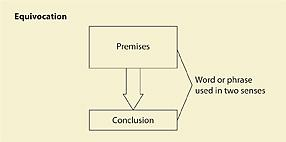
\includegraphics[width=.5\textwidth]{equiv.jpg}
  \end{center}
  
\end{frame}

\begin{frame}
  \frametitle{Equivocation}
  \framesubtitle{Examples}
  
  \begin{block}{Subtle meaning change}
    ``The prosecution contends that my client exited through the window\uncover<3->{$_{opening}$}. But if he had, the window\uncover<3->{$_{pane}$} would have shattered, and the window\uncover<3->{$_{pane}$} was found by police to be intact. Therefore, my client could not have done what they claim.''
  \end{block}
  
    \begin{block}<4->{Structural meaning shift}
    ``George was \alert<5-5>{interviewing} for a \alert<6->{job} drilling oil wells \alert<5->{in the supervisor's office}.  That company is so disorganized.  Why would you drill wells in the supervisor's office?''
  \end{block}
  
\end{frame}

\begin{frame}
  \frametitle{Amphiboly}
  
  \begin{block}{Ignoring the intended meaning}
    \begin{itemize}
      \item Amphiboly also makes use of the ambiguity of certain words and phrases.
      \item The arguer latches onto one possible interpretation of a statement, while ignoring the more plausible, or intended, interpretation.
      \item We may respond to such arguments with, ``That may be what he \textit{said}, but it's not what he \textit{meant}.
    \end{itemize}
  \end{block}
  
  \begin{block}<2->{Example}
    ``Mrs. Hart stated in her will, `I leave my 500-carat diamond necklace and my pet chinchilla to Alice and Theresa.' Therefore, we conclude that Alice gets the necklace and Theresa gets the chinchilla.''
  \end{block}

  
\end{frame}


\section{Fallacies of illicit transference}

\begin{frame}
  \frametitle{Composition and division}
  
  \begin{block}{Parts to whole}
    \begin{itemize}
      \item Reasoning by composition involves looking at the properties of the \textit{parts} of some object, and inferring that the \textit{whole th}ing also has those properties.
      \item For some properties, this is a reasonable conclusion.
      \item But the transference from parts to whole doesn't hold for all properties.
    \end{itemize}
  \end{block}
  
  \begin{block}<2->{Whole to parts}
    \begin{itemize}
      \item The flipside of composition is \textbf{division}.  It involves looking at the properties of the whole, and inferring that the individual parts also have those properties.
      \item Just like composition, some properties transfer from the whole to its parts, but some do not.
    \end{itemize}
  \end{block}
  
\end{frame}

\begin{frame}
  \frametitle{Composition}
  \framesubtitle{Examples}
  
  \begin{block}{Good composition}
    ``As humans, every one of our parts is physical, so it follows that we, too, are physical.  The idea of a soul is a fantasy.''
  \end{block}
  
  \begin{block}<2->{Bad composition}
    ``If given the choice, I would want to carry 100 pounds of feathers rather than 100 pounds of bricks.  After all, feathers are light!''
  \end{block}
  
\end{frame}



\section{Next meeting}

\begin{frame}
  \frametitle{What's coming up?}

  \begin{block}{Jumping into deduction}
    \begin{itemize}
      \item We will start our investigation of formal logic.
      \item We'll indtroduce the notion of argument forms and propositional variables
      \item Relevant readings: \S\S 4.1-4.2
      \item Homework \#2 will be made available on Friday, and is due on Thursday (10/02).  It will cover informal fallacies.
      \item Homework \#1 will be returned on Monday.
    \end{itemize}
  \end{block}
  
\end{frame}

\end{document}
